\documentclass[10pt, journal]{IEEEtran}
\usepackage{graphicx,latexsym}
\usepackage{longtable}
\usepackage{fullpage, setspace} %an example of how to specify two packages at once.
\usepackage[nottoc]{tocbibind}
\usepackage{textgreek}
\usepackage{enumitem}
\usepackage{listings}
\usepackage[T1]{fontenc} % optional
\usepackage{amsmath, nccmath}
\usepackage[most]{tcolorbox}
\usepackage[cmintegrals]{newtxmath}
\usepackage{bm} % optional
%\renewcommand{\arraystretch}{2}

\lstset
{ %Formatting for code in appendix
    basicstyle=\footnotesize,
    numbers=left,
    frame=single,
    xleftmargin=2em,
    framexleftmargin=2.5em,
    %stepnumber=1,
    showstringspaces=false,
    tabsize=1,
    breaklines=true,
    breakatwhitespace=false,
}

\makeatletter
\def\lst@makecaption{%
  \def\@captype{table}%
  \@makecaption
}
\makeatother

\title{Multicast Protocol Verification: Expanding Real-Time Maude Testing to Analyze the NACK Oriented Reliable Multicast Protocol}
\author{Caleb Bowers}
\date{12-13-2019}

\begin{document}

\maketitle
\begin{abstract}
Verification of communication protocols traditionally focused on single channel transmissions and has only recently expanded to evaluate multicast channel protocol verification. These protocols are increasingly useful and necessary in a continually distributed computing and communication environment, both within the Internet and in mobile ad-hoc networks. I examine the formal specification of the NACK Oriented Reliable Multicast (NORM) protocol within the verification and logical framework Real-Time Maude. After replicating initial specification tests and analysis based on system simulation, Linear Temporal Logic (LTL) formulas, and state space search approaches, I devise a framework to expand these analytical approaches using Python and a standardized configuration file. Using this framework, I am able to more extensively test the NORM Real-Time Maude model and provide additional insight into its structure. 
\end{abstract}

\section{Introduction}
In the past thirty years researchers have produced significant improvements in how formal methods are used to verify computer networking protocols. Traditionally, during development and implementation, the protocol would undergo extensive testing as the primary method of verifying that the function of the protocol matched the design specification. If the protocol behavior mirrored that of the design specification, then researchers and designers felt confident enough to label the protocol ``verified,'' or at least stable enough for reliable use. This approach does not concretely verify the protocol, but does prevent obvious errors from existing and can come close to ensuring functionality in expected operational conditions. Extensive testing, however, only verifies the behavior of the specification for the specific domain tested, and does not logically verify the specification itself.

Extensive testing methods work fairly well for day to day unicast Internet protocols where the operating conditions are more predictable and the implementation less complex. There exists a gap, however, for multicast and broadcast networking protocols (hereafter, multicast\footnote{It should be noted that multicast is a subset of broadcast. Broadcast entails a sender transmitting to all network participants, whereas multicast describes a sender transmitting to a \textit{subgroup} of participants.}) and researchers have sought to develop more rigorous formal methods for these networking protocols. 

In multicast environments the participants are often widely distributed and senders only know the group address, rather than the address of each participant (as is the case in unicast). The multicast communications paradigm requires more complex reliability and transmission mechanisms in order to ensure that the protocol maintains efficient use of network resources (e.g, bandwidth). Implementing these mechanisms leads to an explosion of state space, which further limits the efficacy of extensive testing, since that is often domain specific and is limited in time by the number of actual testable domains. Additionally, as previously mentioned, a specification may produce proper behavior amidst most operational conditions, but still not be functionally guaranteed to match the design specification, so a possibility for error exists somewhere in the behavioral domain for that protocol. Formally verifying these complex multicast mechanisms, therefore, remains necessary and is increasingly important as more communication becomes distributed and asynchronous across multicast protocols.

The focus of this paper is to replicate and build off of previous verification efforts that sought to formalize an early, ambiguous draft version of the NACK Oriented Reliable Multicast Protocol (NORM) using the verification framework Real-Time Maude \cite{Lien2004, rfc5740, rtmaudeUrl, maudeUrl}. NORM provides reliable multicast communication amidst even significantly degraded network resources and leverages novel information theoretic methods to recover message information at the bit level, making it the state-of-the-art in reliable multicast communication. In order to provide these delivery guarantees, NORM's design is fairly complex due to its use of Forward Error Correction (FEC) codes, its internal timing methods, and its NACK (negative acknowledgement) based reliability guarantees. Its reliability guarantees make it a desirable protocol to use for multicast applications, but its complexity could make it susceptible to failure, since the state of operation can become easily obfuscated by the large functional state domain, especially as the network increases in size. The initial work focused on specifying and verifying only two of the more approachable, yet still certainly complex, components of the protocol: the local and global round trip time calculation and the data and repair transmission algorithms. 

The goals of this paper focus on replicating and expanding the verification of the data and repair transmission component of the NORM protocol specification to provide a more comprehensive understanding of the Real-Time Maude NORM model. I achieve this by expanding the original testing scenarios and creating a testing generation framework to provide improved systematic testing, thus enabling a better understanding of the computational and time requirements needed by the Real-Time Maude implementation in order to verify/produce a result. The resulting work produces an analysis and regression testing framework that enables the addition of results-driven improvements to the Real-Time Maude NORM model. Additionally, a user may formalize a custom implementation of NORM and then compare results to the baseline Real-Time Maude specification or more rigorously analyze their new specification beyond a small sample of initial state spaces for error and model timing analysis. 

\section{Related Work}
Multicast protocols enable a sender to communicate with a group of receivers simultaneously, and as such, require a higher level of complexity when attempting to provide reliability and security guarantees. While multicast protocols in design may be more complex than unicast communication paradigms, the approaches to their verification do not differ that significantly and a body of literature exists for general protocol verification dating back to the late 1970's \cite{Bochman1980}. A brief overview of some of the significant literature regarding the verification of both multicast protocols is provided before delving into background material.

\subsection{Multicast Protocol Verification}
As previously mentioned, multicast protocols can be significantly more complex than unicast protocols, since the communication originating from a sender can be destined for an arbitrary number of nodes at send time (as opposed to the lifetime of the packet in a unicast protocol). This complexity not only affects how to verify the underlying design of the communications protocol, but how to ensure certain desirable aspects of a communications protocol: security, wireless resilience, etc.

\subsubsection{Historical Multicast Verification}
Early examples of network protocol verification previously mentioned focused primarily on link level properties between fixed entities (e.g, sender and receiver) leveraging a fixed number of lower layer services and components. This approach does not enable the verification of protocols as they are used in the real world where communications happen between an exponential number of entities across complex protocols that make use of an arbitrary number of lower layer services, unicast or multicast. To account for the arbitrary nature of real protocol operational requirements, the researchers shifted from a strict model checking approach, to a technique that uses induction to prove correctness of protocol specifications and properties \cite{Creese1999}, \cite{Callahan1995} ,and \cite{Baptista1990}.

\subsubsection{Current State of Multicast Verification}
Multicast protocols have seen increased use over the past decade as the proliferation of connected devices, improved wireless communication technologies, and increased connectivity has led to a networking environment more focused on communication between and within groups, rather than point to point communications characteristic of the early Internet. This increase in connectivity and devices has led to an emphasis on creating robust multicast protocols that are both reliable and secure. Wireless technologies further increase the need for security, especially within the multicast framework where there occurs less hand-shaking (in general) between communicating parties. In order to ensure these characteristics are present within a multicast protocol, there is a push to formally verify these protocols, specifically for group-oriented environments and wireless communications. 

Prior to focusing on multicast protocol use in wireless settings, researchers turned to verifying additional security primitives for multicast network communication. The focus turned to verifying a system with an arbitrary number of components (as exemplified by streaming digital signature protocols) as a composition of security verified subprocesses carefully constructed to preserve the security properties of the entire system. This technique sufficiently proves that if each single process in a system satisfies a given single property, the composition of two or more \textit{processes} satisfies the compositions of two or more \textit{properties}. Examples using this composition method to demonstrate security satisfiability in multicast protocols are \cite{Gorrieri2008}, \cite{Martina2015}, \cite{Bella2002}, and \cite{Archer2002}.

The emphasis within the field of multicast protocol verification quickly shifted to wireless settings as technological improvements enabled mass communication across the medium. Of particular interest is the functionality of wireless multicast protocols in sparse and poorly resourced networks, generally called edge networks. Analysis of the MobiCast protocol provides an example of verifying a multicast protocol designed to operate within this sparse networking context \cite{Tan2000}. To verify this protocol, the authors develop a model of its functionality within the Prolog language and test this model for a variety of specification properties (i.e., the protocol operates in the way the design specifies) and safety properties (i.e., the protocol operates when it needs to). 

Most wireless multicast research is focused on the development of new and efficient multicast protocols, leaving the verification until later. One additional example is \cite{Anastasi2000}, which examines the verification of a multicast protocol used to coordinate distributed mobile computing processes. The authors use the Calculus of Communicating Systems \cite{Milner1989} and the Concurrency Workbench tool \cite{Cleaveland1996} to specify and verify their mobile computing multicast protocol. Prior to the work being replicated in this paper, NORM had not been formally specified or analyzed, but sees wide use both in wireless contexts and in secure communication environments, so formal analysis of NORM's functional correctness would benefit a large group of users and networking contexts. I wish to expand and improve a framework for testing the Real-Time Maude specification, which will enable

\section{Background}

\subsection{Real-Time Maude}

For communication protocols, time is inherently useful in constructing a communication paradigm and ensuring appropriate steps are taking in exchanging information. Since communicating nodes have no means of knowing whether a message will eventually arrive at its intended recipient, time plays a crucial role in helping nodes determine how to react to the receipt, or lack thereof, of a message/information when participating in a communication session. For example, if a node expects a reply to a previously sent message, it may set a timer to determine how long to wait for that reply before re-sending the message or moving ahead in a communication sequence \cite{Lien2004}.

Within the realm of computing there exists a subset of computing systems whose functionality depends on the passing of time in a real-world setting. These systems are referred to as \textit{real-time} systems as their execution is tightly coupled to the passage of ``real'' time. Within this context, communication protocols constitute such systems, and NORM in particular, heavily leverages and depends on the passage of time for proper functionality. In order to approach the verification of such a protocol, a modeling tool requires additional mechanisms to address the timing constraints a real-time system experiences. The author in \cite{Lien2004} made use of the real-time specification language and analysis tool \textit{Real-Time Maude} \cite{rtmaudeUrl, Olvezky2004}. Real-Time Maude extends the foundational specification language \textit{Maude} \cite{maudeUrl, Clavel2002} based on a logic for modeling concurrent exchanges and evolution in distributed systems called re-write logic \cite{Meseguer1992}. Real-Time Maude enables the user to specify exactly how the change in a concurrent system depends on time. What follows is a high -level view of the theory behind Real-Time Maude, since for the purposes of this project and paper, knowing that Real-Time Maude can be used to specify, analyze, and verify real-time systems, such as NORM, suffices.

Real-Time Maude allows the user to analyze a specification of their system in the Maude language by:
\begin{itemize}
	\item \textit{Simulation}: User can specify a single behavior to simulate through the system specification
	\item \textit{Exhaustive Search}: Real-Time Maude can search through all possible system states for infinite or bounded time from some initial state looking for safe or unsafe states (based on desired property)
	\item \textit{Model Checking}: Using \textit{Linear Temporal Logic Formulas} Real-Time Maude verifies that from some given initial state the system satisfies the formula for all states or up to some time bounded set of states.
\end{itemize}

\subsubsection{Examples of Maude and Real-Time Maude}

Maude has been used recently to verify the YubiKey authentication framework, which is a type of two factor authentication used to authenticate user identity for network-based services such as remote login or file server access \cite{Escobar2018}. Additionally, Maude has a variety of application domains and has been used to verify programming languages (e.g., Java), analyze biological processes and entity interactions, and develop efficient and generally fault-free business production processes (i.e., operations management). 

Real-Time Maude has not seen as wide spread use as its parent program, but has been applied in a variety of fields, though primarily in the realm of communication protocols (making it well-suited to tackle NORM). Researchers have leveraged Real-Time Maude to specify and formally analyze the \textit{optimal geographical density control} algorithm used to coordinate nodes in a wireless sensor networks and the real-time updating, cost-aware scheduling algorithm CASH \cite{Thorvaldsen2007, Caccamo2006}.

\subsubsection{Using and Analyzing Real-Time Maude}

Maude leverages rewrite logic (a set of conditional and unconditional logical deduction rules) to create specifications for systems in order to perform formal analysis and verification of the state behaviors of those systems \cite{Meseguer1992}. Likewise, Real-Time Maude further extends the theory of rewrite logic to encompass time dependent systems and executions by including syntax to specify the time constraints on a Maude command. A simulation of a specific behavior of a system can now be bounded for set time or can be simulated without a time constraint, allowing Maude to find unsafe states/behaviors for real-time systems. Additionally, Real-Time Maude enables time specifications for state space search methods and for evaluating linear temporal logic formulas. This enables users to evaluate time itself as a possible failure cause for system behaviors, which directly impacts functionality of a real-time system (such is the case for NORM).

\subsection{NORM}
In computer networking communication and protocol verification, communication is broken into three main paradigms
\begin{itemize}
	\item \textit{unicast}: A sender transmits to a single receiver. Internet protocols operate on this model.
	\item \textit{broadcast}: A sender transmits to all nodes on the network. This is how computers find printers on a local subnet.
	\item \textit{multicast}: A sender transmits to a subgroup of nodes on the network.
\end{itemize}

Multicast communication enables a sender to transmit a message to a specific group address, or a multicast address \cite{Lien2004}. Once the message is transmitted to this address, delivery of the message to every member of the group depends on the multicast network protocol. When specifying requirements for a multicast protocol, reliability is often provided by balancing the tradeoffs of feedback/retransmission strategies with the ability to scale to a large number of nodes across a wide network. If the protocol creates too much traffic, it will not scale well on its own as a communications protocol, nor will it be useful in larger networking contexts where the multicast protocol must share resources with other communication protocols.

Multicast is, at this point, incredibly popular for a variety of Internet level applications: distributed chat, online video games, and the pushing of software updates. Historically, in order to implement these services, a specialized multicast protocol would have be to be developed or cobbled together using the Internet Protocol stack in a specific manner. With the development of NORM, a lot of the complexity in early multicast implementation was removed, especially for the application uses often leveraging multicast: streaming, file transfer, distributed communications. NORM \cite{rfc5740} combines these application services into a transport layer protocol, which removes the need for the application layer to manage the multicast communication and communicate as it would using any Internet Protocol (e.g., UDP, TCP, etc.). Additionally NORM provides service guarantees amidst degraded network conditions or sparse networking environments by focusing on preventing, detecting, and correcting errors as they arise.

NORM can prevent errors due to congestion control by adjusting sender transmission rate in an adaptive manner and using reduced receiver feedback messages, thus preventing the network from being taxed by unnecessary control messages. In order to detect errors, NORM sequences each packet and the receiver can inform the sender of a successful receipt of data or a need to repair received data. Finally, NORM employs novel FEC encoding to correct errors at the receiving end of the packet, but if this is not enabled, the sender can retransmit lost or damaged packets.

\subsubsection{NORM Overview}
The development of NORM began as an Internet Engineering Task Force (IETF) Internet-Draft and has evolved into a full-fledged Internet Standard in the Request For Comments 5740 \cite{rfc5740} in 2009. In \cite{Lien2004}, whose work I am replicating and seeking to expand, the author used an early draft of NORM that became obsolete in 2003, so room exists to update her work and examine how her Real-Time Maude specification reflects the current Internet Standard specification of NORM. The goal of NORM is to provide reliable, efficient, scalable, and robust transport of large amounts of data over an IP multicast network. To this end, NORM employs:
\begin{itemize}
	\item \textit{NACK based packet repair}: Receivers request repair of packets via a negative-acknowledgement (NACK) when they encounter packet loss
	\item \textit{Reduced receiver feedback}: Receivers are not required to acknowledge receipt of every packet
	\item \textit{Congestion Control}: As mentioned, both sender and receiver can adjust transmission rates to account for network traffic load
\end{itemize}

The main subject interest and analysis will be the data transmission component of NORM, which is responsible for the transmission, delivery, and repair of packets transmitted from sender to receivers. These data transmitted can be objects (i.e., messages broken into packets/datagrams) or "infinite" streams of data marked with an object identifier unique to streams. NORM accomplishes the transmission of these objects using the following messages:

\textbf{Sender}
\begin{itemize}
	\item \textit{NORM\_DATA}: Used for sending and retransmitting data segments (depending on internal flags) from the application layer
	\item \textit{NORM\_CMD}: Control messages in NORM to administer operation.
	\begin{itemize}
		\item \textit{NORM\_CMD(CC)}: used to monitor network congestion and establish round trip times for receiver group(s)
		\item \textit{NORM\_CMD(FLUSH)}: Once the sender transmits this message, the receivers know that it is preparing to flush (delete) queued data and repair segments, which means receivers must submit any remaining repair requests if they wish to recover lost data
		\item \textit{NORM\_CMD(SQUELCH)}: Senders transmit this message to all receivers if the sender has received a repair request for data it can no longer repair. This message provides information about which data objects are still eligible for repair
	\end{itemize}
\end{itemize}

\textbf{Receiver}
\begin{itemize}
	\item \textit{NORM\_NACK}: Used to request repair of lost or incomplete data segments
	\item \textit{NORM\_ACK}: Used to acknowledge NORM\_CMD messages from sender
\end{itemize}

The sender messages \textit{NORM\_DATA}, \textit{NORM\_CMD(FLUSH)}, and \textit{NORM\_CMD(SQUELCH)}; and both receiver messages are used in the data transmission component of NORM, which I will be modeling and analyzing in Real-Time Maude. There are three sections in the transmission and repair of data: sender transmission (\textit{NORM\_DATA}, receiver repair request (\textit{NORM\_CMD(FLUSH)}, \textit{NORM\_NACK}), and sender NACK processing/repairing (\textit{NORM\_CMD(FLUSH)}, \textit{NORM\_CMD(SQUELCH)}).

\subsubsection{NORM Specification and Model}
The Real-Time Maude specification model does not include components for congestion control, since this functionality is not crucial to ensuring reliability, but exists to relieve excessive network traffic. This specification further models communication with one sender to arbitrarily many receivers (\textit{one-to-many}). While NORM can support arbitrarily many senders to arbitrarily many receivers, most actual implementations leverage a \textit{one-to-many} paradigm (e.g., pushing a software update), so this is most beneficial to analyze. Additionally, all communication between senders and receivers is multicast\footnote{NORM can operate with transmission multicast from sender and the receivers have a unicast channel back to the sender}. Only finite data objects (e.g., messages, file transfers, etc.) will be examined without the use of FEC codes (these are used for packet recovery and do not affect instantiated NORM session communication between sender and receivers\footnote{An instantiated NORM session cannot add FEC encoding midway, but must have this specified beforehand. Of course, FEC encoding will reduce the amount of repair requests, so communication between senders and receivers would be impacted, but within the already defined NORM communication paradigm.})

Additionally, the following assumptions are made in the Real-Time Maude specification:
\begin{enumerate}
	\item Though NORM can operate within dynamic mobile contexts, only static topologies will be considered (for ease of analysis)
	\item Time will progress in the Maude analysis only when those NORM objects and components specified are operating in time, hereafter referred to as NORM time (e.g., packet transfer will consume time, but instantaneous actions, such as packet wrapping for transmission, will not). 
	\item The random backoff timeout algorithm, which is critical to the receiver transmitting NACK repair requests and in distributing the round trip time calculations on a per receiver basis has remain unchanged in updated design specifications of NORM.
\end{enumerate}

\section{NORM Data and Repair Transmission Component}
What follows is an explanation and some brief detail of the Real-Time Maude specification for the data transmission component of NORM. The author in \cite{Lien2004} originally had some difficulty in discerning particular sections (to be highlighted) due to ambiguity in the IETF draft specification. Fortunately, the ambiguities identified by the author have all been resolved in the updated specification.

\subsection{Specification}
The author of \cite{Lien2004} identified three areas of ambiguity in the IETF draft version of NORM that required her to make a decision on how the specific ambiguous piece of NORM functionality would be modeled in Real-Time Maude. Her decisions were additionally informed by the designers of NORM and updated versions of the NORM specification as they were released at the time of her authorship. The author identified the following areas as underspecified or ambiguous:
\begin{enumerate}
	\item \textit{Receiver NACK Cycle Initiation}: Normally, a NORM receiver will initiate the NACK cycle at specific events: NormObject boundaries, FEC coding block boundaries, or receipt of NORM\_CMD(FLUSH) messages. An alternative, self-initiating NACK cycle option also exists for receivers when no data is currently being received from a sender. The original IETF draft provides no details on this self-initiating NACK cycle process. Updated versions of the NORM standard, however, do provide detail on this operation and specifying this behavior will consitute part of my results.
	\item \textit{Sender NACK Accumulation Timeout}: This ambiguity arose from a discrepancy between the 2003 NORM IETF draft document and the NORM building blocks document \cite{rfc5401}. The timeouts were specified differently in the two documents, and the IETF draft listed timeout did not allow for the receiver feedback suppression algorithm timeout to expire. This was corrected at the time of her original drafting of the Real-Time Maude specification.
	\item \textit{Sender FLUSH Process}: The IETF draft of NORM ended the request and repair process between senders and receivers via a flag (NORM\_FLUSH\_FLAG\_EOT) embedded in the NORM\_CMD(FLUSH) message. This is the same message that informs receivers to request repairs, so it is unclear that if a receiver receives a NORM\_CMD(FLUSH) message with the flag set to end transmission that it would have time to submit last minute repair requests. This problem is remedied in the current version of NORM by forcing the sender to wait for a timeout period of 2 times the greatest round trip time after sending the final NORM\_CMD(FLUSH) message with the flag turned on, which allows it to receive any remaining repair requests from receivers.
\end{enumerate}

The data transmission component is broken up into two classes for the Real-Time Maude specification: \texttt{DTsender} and \texttt{DTreceiver}, which inherit from the base classes Sender and Receiver, respectfully. An application layer module, \texttt{APPLICATIONS}, defines applications to send and receive data. The sender application enqueues data for transmission and the receiver application collects data received by the receiver node \cite{Lien2004}. The author further defines an \texttt{OBJECT} message, which will be a "base" message that the other message types will "inherit" (i.e., wrap) for the different types of NORM messages defined. The following messages are defined for the data transmission component: NORM\_DATA, NORM\_CMD(FLUSH), NORM\_CMD(SQUELCH), and NORM\_NACK. 

In Real-Time Maude, rules define the behavior of a system on the Maude objects that the model comprises. The author originally defined several rules for \texttt{DTsender}:
\begin{itemize}
	\item The transmission of new data content
	\item The flush (e.g., repair request) process
	\item The NORM\_NACK accumulation period
	\item The repair of data transmission
	\item Timeout to accept repair requests
	\item Notifying receivers of invalid repair requests. 
\end{itemize}
\noindent
Rules defined for \texttt{DTreceiver} consist of:
\begin{itemize}
	\item The initiation of the NACK cycle at NormObject boundaries
	\item NACK cycle initiated by receipt of NORM\_CMD(FLUSH)
	\item Repair message reception
	\item Forwarding data up to application layer
	\item Accumulating external repair requests from other receivers to forward to sender node
	\item Transmitting repair request after holdoff timeout
	\item Cancel invalid repair requests
\end{itemize}

The previous classes, modules, and rules are required in Real-Time Maude to formally analyze and verify a system using the Maude/Real-Time Maude framework. Once these system components are defined, the system can be evaluated by defining a variety of initial states from which property satisfiability and system correctness can be analyzed. These states will be defined in the Analysis section.

\subsection{Analysis Replication}

Several hurdles were encountered when attempting to replicate the analysis of the data transmission and repair component using the original Real-Time Maude specification from \cite{Lien2004}. I had to replicate a testing environment used in the early 2000's on my current operating system and hardware that is the result of almost twenty years of constant technological improvement. The following steps were required in order to replicate the analysis from the original Real-Time Maude investigation.

The author used Real-Time Maude 2.0, which was released in in 2004 and operated on top of Maude 2.0 (released in 2003). Locating Real-Time Maude 2.0 was not too difficult and only consists of a Maude file that defines the timing mechanisms for real-time analysis. Maude 2.0 proved somewhat more complex. Initially, I attempted to build version 2.0 from source, but was continually met with compiler errors that resulted from significant changes in Linux c compiler design over the past 16 years. Eventually, I located a pre-built unix binary that I was able to execute on my Linux system and I only needed to invoke this binary with the Real-Time Maude 2.0 definitions file in order to run Real-Time Maude. Maude 2.0, however, could not run initially within my terminal, since it contained too many color options and additional graphics options that Maude did not know how to parse. This was easily remedied by downloading a vt100 terminal emulator: xvt. Within xvt I was able to execute Real-Time Maude and run some example tests from the distribution website \cite{rtmaudeUrl}.

The next hurdle involved implementing the Real-Time Maude specification of NORM in my Real-Time Maude environment. Initially, I attempted to copy the entire specification from the appendix of \cite{Lien2004}, but this proved to be an incomplete specification and lacked the object-oriented architectural structure required by the Real-Time Maude methods. Eventually, I found the author's code in an online repository of Real-Time Maude use cases. I was able to execute her files after some minor commenting and syntax errors (statements, both in Maude and Real-Time Maude require termination with periods, some of which were missing from the files in the repository. The files seemed to be in a state of mid-completion/mid-testing, so were not completely polished.) After cleaning up the coding errors, I began replicating the tests the author developed in her initial Real-Time Maude analysis of NORM.

\subsubsection{Data and Repair Properties}

The author defined several properties for her analysis of the data and repair component of NORM ranging from examining initial sate behavior to assessing LTL logic formulas on the system. The following properties were defined for the data and repair component and I successfully replicated all of them within my Real-Time Maude environment.
\begin{figure}
	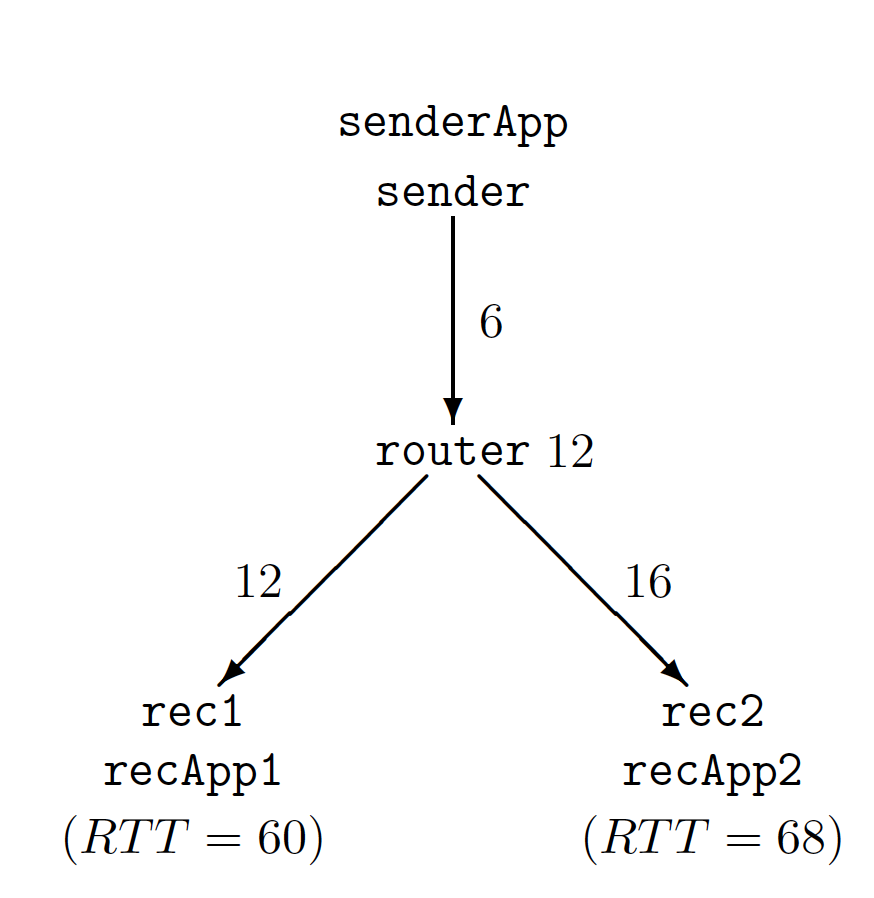
\includegraphics[width=\linewidth]{../DT_Topo1.png}
	\caption{\texttt{data1} Topology}
	\label{fig:data1}
\end{figure}

\begin{itemize}
	\item Initially, a network topology and an initial state were defined and referred to as \texttt{data1} (see figure \ref{fig:data1}). Within this network and topology, 4 data objects of 70 data segments are being transmitted from \texttt{sender} to the two receviers: \texttt{rec1} and \texttt{rec2}. The \texttt{sender} node transmits through a router node and the links between all of these nodes have an associated delay which will impact the performance of NORM and should be captured within the Real-Time Maude analysis.
	\item The first analysis I attempt to replicate simply determines whether NORM will converge (receivers receive all data segments) for the initial state of \texttt{data1}. This takes the form of an unbounded rewrite command that simply simulates the system until it terminates: \texttt{(trew data1 with no time limit .)} (where trew is the timed rewrite command in Real-Time Maude). In both the original implementation in \cite{Lien2004} and in my Real-Time Maude environment the system converges with all segments delivered in 4,240 NORM timed operations.
	\item Having established this topology as a valid NORM transmission state space, I turn my attention to replicating the searching of the state space. Though the simulation produced a state where transmission successfully converged, it is only one behavior, not all possible states. The state space must be searched for erroneous behaviors, such as a state where the sender receives a repair request having already completed its transmission session (the sender only completes sending when it believes the receivers have finished submitting repair requests). A state space search of 5000 NORM timed operations is conducted, but is ultimately aborted, because the search fails to complete within reasonable time. This results from significant nondeterminism within the NORM specification, so the state space explodes as time progresses; therefore, 5000 timed operations becomes infeasible to search. Reducing the timed operations to 350, produces a safe state space; that is, no states are reached where a sender receives a repair request having already completed transmission. My analytical expansion will enable more extensive testing to reveal the system time that produces the earliest Real-Time Maude execution that requires aborting.
	\item The next stage of analysis involves creating a model checker for NORM that defines three atomic propositions (evaluates True or False):
	\begin{enumerate}
		\item packetSent: Packet is sent.
		\item packetRec1: Packet is received at receiver 1
		\item packetRec2: Packet is received at receiver 2
	\end{enumerate}
	An LTL formula is then created to evaluate (with respect to initial state \texttt{data1}) the property: it is always true that if a packet, x, is sent, it will eventually be received by both receivers. In standard LTL syntax, this would read:
	\begin{equation}
	\begin{aligned}
		\square(PackSent(x) \implies \\ 
		(\lozenge packetRec1(x) \wedge \lozenge packetRec2(x)))
	\end{aligned}
	\end{equation}
	The original analysis executes this statement for the first ten data segments within NORM time 200 after the author used Real-Time Maude to determine the longest NORM time it could take for the first ten segments to be delivered: NORM time 150. Executing the previous LTL formula on the first ten segments returns true for all ten cases. It is important to remember that this true result only holds with respect to the initial state \texttt{data1} on the first 10 data segments (there are a total of 280), and in most circumstances there are nearly infinite number of initial states and configurations, so verifying this component on this specific LTL formula is time prohibitive. But, this analysis does enable the locating of errors that may not be exposed via functional testing. As part of my analytical expansion, I will be examining this specific analysis to provide a framework for generating the scripts to quickly run a Real-Time Maude analysis on all data segments rather than writing each data segment command by hand.	
	\item The final analysis examines an updated topology and initial state: \texttt{data2}, which is graphically identical to \texttt{data1}, but the initial state increases the router queuing delay. Increasing this delay further increases the state space of the system, so exhaustive state space search is even more infeasible, so analysis is restricted to rewrite simulation. A simulation of transmission on \texttt{data2} produces a state where neither receiver is able to receive all of the data segments. The receivers fail to receive all of the data segments, because the router queuing delay prevents the sender from receiving the repair requests from the receivers. Since the sender does not know there are additional repair requests, it assumes the receivers have received all of the data segments and ends the transmission. This situation would ideally be avoided or overcome by NORM, and the results of this analysis improved how the NORM sender terminates a transmission session by adaptively changing the timeout for control and repair messages to account for increase delivery delay.
\end{itemize}

I was able to fairly straightforwardly replicate the results from the original investigation in \cite{Lien2004}, though by the author's own admission, the analysis of the data and repair transmission is incomplete and could be expanded. The expansion of this analysis constitutes the second part of my contribution to this work.

\subsection{Expanding Analysis}

\subsubsection{Expanded Testing Framework}
The original analysis of the Real-Time Maude model of the NORM protocol sufficiently demonstrated the capabilities of Real-Time Maude to analyze an asynchronous protocol such as NORM and produce results that could be used to improve a design specification. This analysis, however, really only provides insight into the potential design considerations and does not provide much insight into the structure of the system or how the progression of time may affect the proper functioning of the protocol. In order to arrive at such results, the analysis must be expanded to be more extensive. For example, it is much more valuable as a system designer/verifier to know at what point in execution time the state space becomes infeasible to search and how the state space has progressed to that point, rather than simply knowing that at system time 5000 the state space is too large to search. 

Extensively testing a Real-Time Maude specification, however, can be difficult, time-consuming, and error prone, since a user must hand-write all of the initial state values, the model checking properties, and then write the Real-Time Maude analysis commands on top of all of that. In an attempt to alleviate this testing burden, so extensive testing can be performed, I have developed a testing framework to quickly generate user specified state space, simulation, and LTL formula evaluation statements to be used in a Real-Time Maude model evaluation. The framework is constructed using a script written in Python 3.5 and makes use of a user generated configuration file, named \texttt{rtmaude.config} (or any name the user desires)\footnote{Code is available upon request}. The script, \texttt{write\_rtmaude.py}, parses the config file for general test settings and then settings specific to simulation, LTL formula testing, and state space search testing. It is important to note that a user must already have a Real-Time Maude system model generated in order to make use of this tool.

Four sections comprise the configuration file:
\begin{enumerate}
	\item $<$test$>$: These settings are general to the Real-Time Maude evaluation, such as topologies involved, the files that defines the Real-Time Maude model, and the name of testing output file.
	\item$<$tsearch$>$: This section contains settings specific to generating state space search statements, such as topology/start state to search and a list of times to limit the search.
	\item $<$trew$>$: These settings are specific to simulating a behavior in the Real-Time Maude model, namely, start state and length of simulation.
	\item $<$ltl\_form$>$: LTL formula settings are listed here. These settings must refer to atomic operations defined in a Real-Time Maude specification file (set in the $<$test$>$ section). These settings include a list of times to evaluate, number of start states, etc.
\end{enumerate}
As one can see from this list, the sections are specified within the configuration file as beginning with $<$section\_name$>$ and the sections end with $<$/section\_name$>$ similar to XML style formatting. Once these parameters are set, a user can execute the \texttt{write\_rtmaude.py} script on the configuration file and quickly generate the statements needed to more thoroughly test desired Real-Time Maude specification. This framework provides enough flexibility to increase the number of basic tests, but future work remains to make it truly usable by a wide range of researchers and adaptable to different verification contexts, not just the NORM Real-Time Maude specification.

\subsubsection{Expanded Testing Approach}
Building off of the original evaluation detailed above, the areas where additional testing can be performed is searching the state space starting from the initial state \texttt{data1} and further evaluating the LTL formula testing transmission and delivery guarantees (equation 1). With this in mind, I had two goals to add to the evaluation of the NORM Real-Time Maude model:
\begin{enumerate}
	\item Determine more definitively at what point in time the state space becomes infeasible to search for a behavior where (with respect to initial state \texttt{data1}) one or both receivers do not receiver all of the data segments transmitted. The author mentioned her computer memory as a possible limiting factor. Presumably, in 2004 her machine possessed at most 512 megabytes of RAM memory, which is about 16 times less than what my machine currently is running, so I should be able to search state spaces at larger time values, though running time is still a limiting factor and could still render searching the state space untenable. Additionally, the author originally looked at state space time search values of 5000 and 350, which creates a large span of time for which little is known about the system. I intend to gain greater insight into this window of time, though the time value for which searching becomes infeasible may not be much greater than the author's original low time value given how rapidly state space can increase.
	\item Evaluate the LTL formula defined in equation 1 for all 280 data segments. That is, determine if for initial state \texttt{data1} the LTL formula holds true for all 280 data segments intended for transfer within system time 200. Some of these will certainly prove false, since the simulation conducted earlier found a path for which the system as whole terminated at NORM time 4,240. Though this is only one example execution for the initial state, it is unlikely that this is a high-side outlier for the system to come to a terminating state. The time limit, therefore, may be what causes the LTL formulas to evaluate false for a given data segment, rather than an error in the protocol. This can inspire additional time testing for those LTL formulas to determine a time for which they all evaluate true.
\end{enumerate}
In order to asses these additional tests, I generated the state space search and LTL formula evaluation commands using my testing framework and then executed the generated commands on the existing NORM Real-Time Maude model.

\subsubsection{Expanded Framework Results}
The LTL formula evaluation for all 280 data segments reached a false evaluation after successfully transmitting 13 data segments within 200 NORM time. To reach this conclusion took 50 minutes 31 seconds for the user and consumed 31 CPU minutes. Real-Time Maude provided a counter example state for data segment 14's failed transmission, but it is over 10,000 lines long (the output file itself is 194 megabytes and over 250,000 lines long for all 266 counter examples, which leads me to believe that a significant portion of the execution time is simply due to the flushing of STDOUT buffers). While a 10,000 line counter example may not be very helpful, it can easily be seen that the formula evaluated false because of the time constraint associated with the LTL evaluation. This demonstrates, however, that Real-Time Maude can be used to simulate an initial state behavior and use that result (4,240 NORM time to converge) to write additional analysis commands, such as evaluating this LTL formula for all 280 data segments within NORM time 4,240\footnote{The time to complete this execution prohibits me from including it in this paper. It remains for future work.}.

Generating the commands to improve the level of fidelity for state space search, proved equally as straightforward within my testing framework. I decided to search the state space for NORM times 100 to 1000 at 50 NORM time intervals. I concluded this would give me a better understanding at which point the time to search a state space becomes untenable, while also giving me insight into the increase in time between each search (Real-Time Maude output provides this information, see Table \ref{table:1}). Executing the commands proved taxing on my machine and utilized 100\% of the CPU for the entirety of its execution, which I ended up having to abort after 2 hours and it having only searched up to NORM time 600. The good news, however, is that no erroneous behavior was found up until this point, and this two hour timeframe does not represent the time spent searching only the state space for time 600, but all of the searches combined. While this iterative testing is interesting, it could be useful for a user to specify in Real-Time Maude a user amount of time (i.e., real world time) to spend searching and after the conclusion of that amount of time, Real-Time Maude could return its system time (in our case, NORM time) evaluation for the state space it has searched. This paradigm though, would be more for user convenience, rather than specific insight into the modeled system since the reference time would no longer be tied to the Real-Time Maude specification, but on the computer being used to conduct the analysis.

\begin{table}[h!]
\centering
 \begin{tabular}{||c c c||} 
 \hline
 System Time & User Time & CPU Time \\ [0.5ex] 
 \hline\hline
 100 NORM Time & .503 s & .504 s \\ 
 \hline
 150 NORM Time & 2.583 s & 2.584 s \\
 \hline
 200 NORM Time& 6.923 & 6.908 s \\
 \hline
 250 NORM Time & 14.500 s & 14.412 s \\
 \hline
 300 NORM Time & 32.795 s & 32.636 s \\ 
 \hline
 350 NORM Time & 68.546 s & 68.296 s \\
 \hline
 400 NORM Time & 163.722 s & 163.408 s \\
 \hline
 450 NORM Time & 351.012 s & 350.988 s \\
 \hline
 500 NORM Time & 952.533 s & 952.444 s \\
 \hline
 550 NORM Time & 1,691.456 s & 1,689.516 s \\ 
 \hline
 600 NORM Time & 3,948.854 s & 3,947.224 s \\[.5ex]
 \hline
\end{tabular}
\caption{Timing statistics for State Space Search}
\label{table:1}
\end{table}

\section{Conclusion}
In this paper I conducted an examination of a Real-Time Maude specification of the NORM multicast protocol. In doing so, I replicated previous results and developed a testing framework to improve and expand Real-Time Maude specification analysis. I achieved this by providing Real-Time Maude users the ability to generate iterative tests for simulation, state space search, and the evaluation of LTL formulas over user-defined properties. This framework can be extended to additional models and I demonstrated that it provides a framework for gaining systematic insight into a Real-Time Maude specification.

\bibliographystyle{IEEEtran}
\bibliography{sem_project_bib}

\end{document}